%%% start preambling . . .  %%%
\documentclass{article}
% required 
\usepackage{amsmath}
\usepackage[semicolon]{natbib}
\bibliographystyle{plainnat} %{unsrtnat}
\usepackage{xr-hyper}
\usepackage{hyperref}
\externaldocument[supplement-]{supplement}
\usepackage{booktabs,siunitx}
\usepackage{Sweave}
\usepackage{graphicx}
\usepackage{lipsum}                     % Dummytext % https://tex.stackexchange.com/questions/9796/how-to-add-todo-notes
\usepackage{xargs}                      % Use more than one optional parameter in a new commands
\usepackage[pdftex,dvipsnames]{xcolor}  % Coloured text etc.
\usepackage[colorinlistoftodos,prependcaption,textsize=tiny]{todonotes}
\newcommandx{\unsure}[2][1=]{\todo[linecolor=red,backgroundcolor=red!25,bordercolor=red,#1]{#2}}
\newcommandx{\change}[2][1=]{\todo[linecolor=blue,backgroundcolor=blue!25,bordercolor=blue,#1]{#2}}
\newcommandx{\info}[2][1=]{\todo[linecolor=OliveGreen,backgroundcolor=OliveGreen!25,bordercolor=OliveGreen,#1]{#2}}
\newcommandx{\improvement}[2][1=]{\todo[linecolor=Plum,backgroundcolor=Plum!25,bordercolor=Plum,#1]{#2}}
\newcommandx{\thiswillnotshow}[2][1=]{\todo[disable,#1]{#2}}
% https://tex.stackexchange.com/questions/60209/how-to-add-an-extra-level-of-sections-with-headings-below-subsubsection
\usepackage{titlesec}
\setcounter{secnumdepth}{4}

\titleformat{\paragraph}
{\normalfont\normalsize\bfseries}{\theparagraph}{1em}{}
\titlespacing*{\paragraph}
{0pt}{3.25ex plus 1ex minus .2ex}{1.5ex plus .2ex}

% recommended! Uncomment the below line and change the path for your computer!
 
%put your figures in one place! Also, note that here 'figures' is the folder and 'demoFig' is what each 
% figure produced will be titled plus its number or label (e.g., demoFig-nqpbetter.pdf')
% make your captioning look better
\usepackage[small]{caption}
\setlength{\captionmargin}{30pt}
\setlength{\abovecaptionskip}{0pt}
\setlength{\belowcaptionskip}{10pt}
% optional: muck with spacing
\topmargin -1.5cm        
\oddsidemargin 0.5cm   
\evensidemargin 0.5cm  % same as oddsidemargin but for left-hand pages
\textwidth 15.59cm
\textheight 21.94cm 
% \renewcommand{\baselinestretch}{1.5} % 1.5 lines between lines
\parindent 0pt		  % sets leading space for paragraphs
% optional: cute, fancy headers
\usepackage{fancyhdr}
\pagestyle{fancy}
\fancyhead[LO]{March 2023}
\fancyhead[RO]{Manuscript}
% more optionals! %
% \usepackage[hyphens]{url} % this wraps my URL versus letting it spill across the page, a bad habit LaTeX has
%%% end preambling. %%%

\begin{document}
\Sconcordance{concordance:supplement.tex:supplement.Rnw:%
1 65 1}
 % For RStudio hiccups
\title{{\huge Changes and trends in budburst and leaf flush across Europe and North America} \\A meta-analysis of local adaptation in spring phenology studies}
\author{Ziyun Zeng \& E. M. Wolkovich}
\date{2023}
\maketitle 


\newpage

\section*{Abstract}


% We conducted the first cross-continental meta-analysis of published studies from the peer-reviewed literature that reported spring event dates for a mix of angiosperm and gymnosperm tree species in the northern hemisphere, capturing data from 384 North American provenances and 101 European provenances with observations from 1962 to 2019.


\section{Introduction}
To optimize ecosystem services for habitat conservation and understand how plants cope with environmental variations, predicting the biological impacts of climate change is of critical importance \citep{botero15}. One of the most important parts of accurate prediction is understanding the relative importance of local adaptation versus plasticity \citep{chevin10}. Local adaptation - how well the growth and adaptive characteristics of plants align with the local climate conditions - influences their ability to thrive and reproduce  \citep{casmey22, kawecki04, anderson12, kim13}. When the selection intensity exceeds gene flow in species that spread over diverse areas, clinal variations among environmental factors can result in populations with unique adaptations to the local climate and, therefore, greater fitness \citep{kremer12, rossi15, salmela13}. On the other hand, phenotypic plasticity describes an individual genotype’s ability to exhibit different phenotypes in response to environmental variations, enabling plants to adjust to new environmental conditions and survive in this rapidly changing world (also known as ‘plastic rescue’)  \citep{chevin10, chevin102, snell18}. \\
\\
Among the various population-level characteristics critical in synchronizing plant growth with the available growing season, phenology traits hold particular significance \citep{primack80, oneil97, chuine01}. Phenology governs the timing of plant transitions between dormancy and active growing, allowing them to time reproduction and utilize each growing season as best as possible \citep{chuine10, hanninen11}. Additionally, phenology provides insight into how climate change affects plant life cycles, regeneration capacity, and ecosystem management.\\
\\
Spring phenology, specifically the timing of budburst and leaf flush, plays a significant role in determining plant fitness and has been widely adopted as a useful tool to investigate plant adaptation mechanisms \citep{guo22, chuine01}. In temperate and boreal environments, the optimal timing for spring growth initiation is determined by a balance of avoiding late spring frost and having a long growing season \citep{alberto11, lenz16, allevato19}. Utilizing the early portion of the growing season can be especially critical for species in colder regions \citep{morin07, dantec15} and the ones with suboptimal shade tolerance \citep{richardson09}. Plants that budburst earlier can take advantage of a longer growing season and avoid competition  \citep{guo22}. \\
\\
In recent decades, there has been growing interest in how climate change influences plant phenology \citep{Gill15}. Trees exhibit immediate responses via phenotypic plasticity with the warming climate \citep{Nicotra10}, while the degree of adaptation dictated by climate change differs across different geographical areas \citep{Loarie09}. Phenological shifts in spring phenology due to recent temperature increases have been extensively observed \citep{Parmesan06}. For example, leaf unfolding in Europe advanced up to six days since the early 1960s due to the rise in spring temperature, and spring events have generally shifted more than fall events \citep{menzel99}. Studies have found that species that shift more with warming also appear to perform better \citep{Gill15}. For instance, research has demonstrated that the timing of budburst and senescence in deciduous plants can impact plant competition \citep{fridley12}, plant growth \citep{myneni97}, and the uptake of carbon by the ecosystem \citep{Barichivich12}. As leaf phenology shifts in response to climate, increasing evidence suggests how much a species shifts its phenology with warming may predict fitness consequences: Individuals, populations, and phenological events (spring versus fall) with more plasticity might fare better with climate change. Plasticity, however, likely varies across species and phenophases. An accurate understanding of how environmental conditions might influence species distribution at a continental scale is critical for future range shift prediction. \\
\\
Much spring phenology is driven by plasticity. For more than 250 years, researchers have been comparing populations of trees from different geographical origins under the same environmental conditions through common garden experiments to disentangle the effects of environmental and genetic variation on trees’ phenology and phenotype \citep{AitkenBemmels16, Alberto13}. Over time, comparable clinal variations have been observed in these experiments along latitudinal and elevational gradients for many temperate and boreal species. Fall bud set phenology and cold hardiness exhibit strong population differentiation and strong clines along different latitudes, altitudes, and continentality gradients \citep{Alberto13}. For example, low-latitude populations have shown significantly stronger delays in leaf senescence over time than high-latitude populations \citep{Gill15}. Spring events (budburst, leaf flush, etc.) show more substantial phenotypic plasticity and higher variability \citep{AitkenBemmels16}.\\
\\
Despite a growing interest in predicting local adaptation across locations, no study has comprehensively examined clines for spring and fall events and what factors may underlie differences observed across studies. We ask: To what extent are patterns of phenotypic plasticity and local adaptation along climate gradients similar across common garden studies? To better understand these clines, we also aim to examine the following:
\begin{itemize}
\item How different are clines between spring and fall phenology? 
\item How different are clines across Europe and North America?
\item If differences in clines exist across angiosperm and gymnosperm species?
\item If climate overlap between the provenance and garden explains the similarities and differences in clines?
\end{itemize}
To address these questions, we reanalyzed data from the literature on common garden experiments in temperate tree species across Europe and North America. 


\section{Methods}
\subsection{Data Collection}
To locate common garden studies that reported the timing of spring events of woody plant species we searched and reviewed the peer-reviewed literature. On 14 December 2022 we searched Web of Science (Thompson Reuters, New York, NY) using the following terms:
\begin{quote}
TOPIC = (common garden* OR provenance*) AND (leafout* OR leaf out* OR budburst OR spring phenolog*)
\end{quote}
which returned 122 publications. We also contacted authors of previous review papers \citep{AitkenBemmels16, Alberto13}, to help further search the literature. We then reviewed the methods and results of all publications to refine to only studies that met the following criteria: (a) focused on woody plants originating from either Europe or North America, (b) had provenance trials/common gardens on the same continent, (c) reported latitude and longitude of provenances and gardens, and (d) reported spring events in units of calendar days (day of year or DOY) or could be converted into DOY (see \nameref{supplement-section:addmethods} in the Supplements).
\\
\\
Based on these criteria we found 19 common gardens distributed throughout North America and Europe, with the majority of data concentrated in North America (Fig. \ref{figure:map_gardens} \& Supplement Table.\ref{supplement-table:all_studies}). From each common garden study we extracted phenological data on spring events (budburst and leaf flush) in DOY and, when present in the same paper, fall events (bud set, leaf senescence, growth cessation, and leaf abscission) by species and the geographic information of provenances and gardens. We used ImageJ (version 1.53k; \citealp{schneider_rasband_eliceiri_2012}) to extract values from figures whenever necessary. For studies that reported event dates relative to a reference date other than 1 January (e.g. \citealp{Rehfeldt1994}), we converted such dates to DOY using the 'lubridate' package in R \citep{Grolemund11}.
\\
\begin{figure}[!h] 
    \centering
 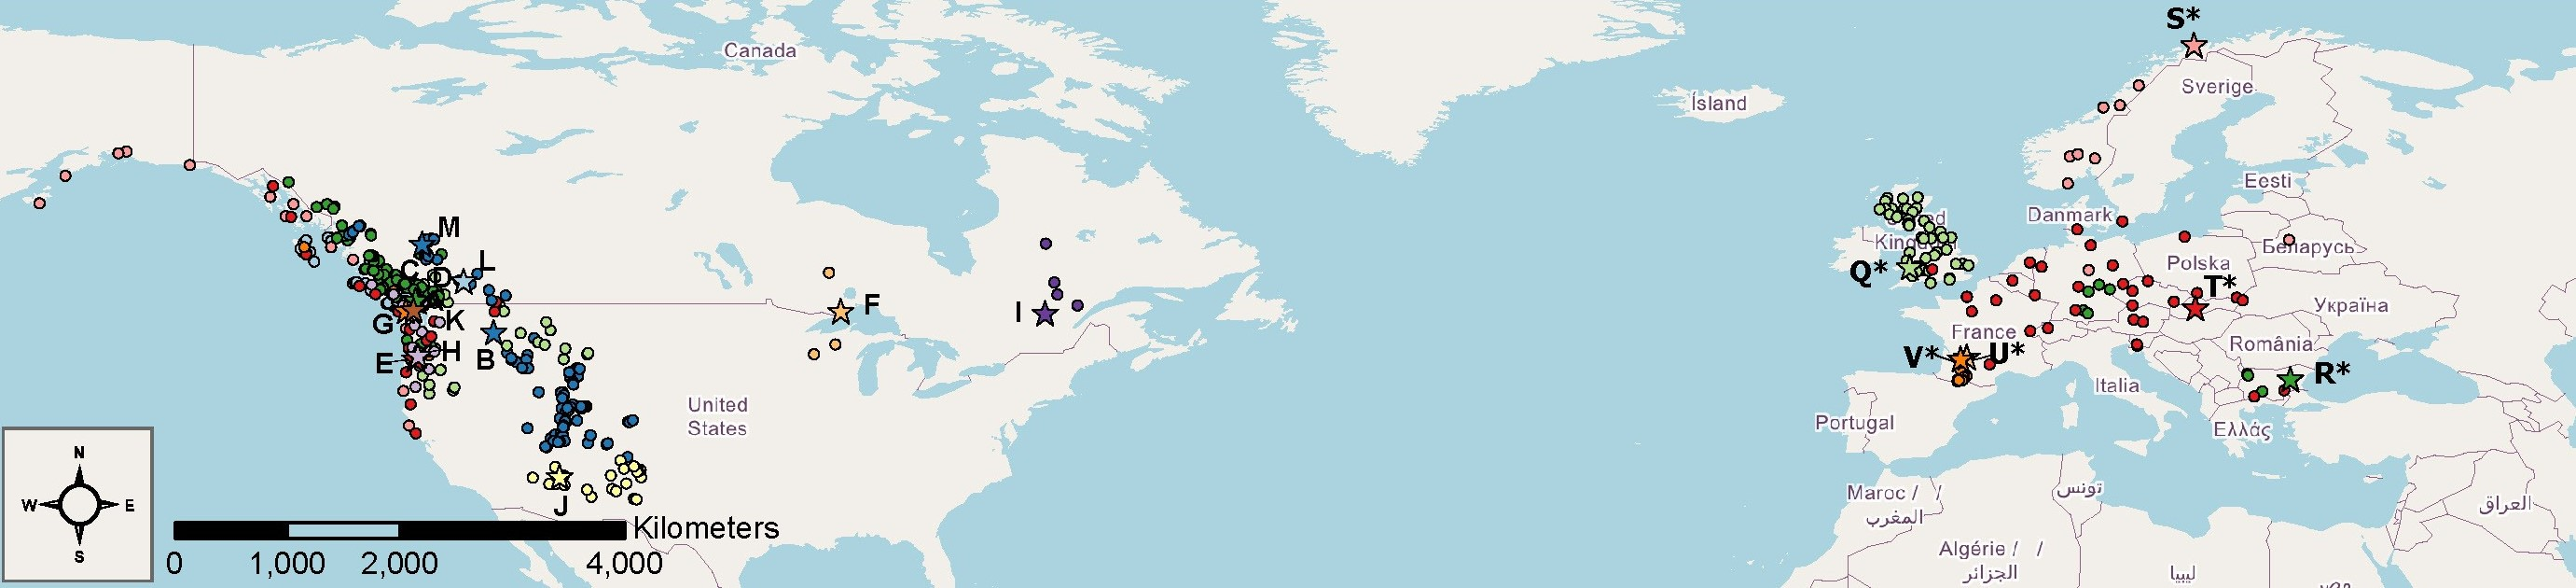
\includegraphics[width=\textwidth]{..//..//localadaptclim/Docs/figure_ms/map_gardens.jpg}
    \caption{Distribution of common gardens (denoted as stars) and provenances (denoted as circles) included in this meta-analysis. The distribution was skewed toward North America (number of studies = 12). See Table.\ref{supplement-table:all_studies} in Supplements for information on selected studies.} 
    \label{figure:map_gardens}
\end{figure}
\newline
To understand how climatic differences, in addition to geographical differences, shape local adaptation in spring events we extracted several types of climate data using information about provenance latitude, longitude, and elevation from original publications. We estimated the mean annual temperature (MAT) for each provenance using the Climate Information Tool by Food and Agriculture Organization of the United Nations \citep{FAO2022}and ClimateWNA \citep{wang2016}. To examine more explicitly climate near spring events, we used gridded daily temperature data for 2011 to 2020 for all European and North American provenances and gardens from E-OBS and the 'daymetr' package in R respectively \citep{cornes2018,hufkens2018}. Using these data we estimated how much the daily temperatures overlapped between garden and provenance locations, which we call `climate overlap.' For this we used the 'overlap' package in R to calculate the percentage overlap of the daily temperature of each provenance and their corresponding gardens in spring months (March to May) from 2011 to 2020. Finally, using the daily temperature data, we also calculated Growing degree days (GDD), a commonly used heat accumulation measure to forecast phenological development in plants (Miller et al., 2001), based on the accumulation of mean daily temperatures ($T_{m}$)from 2011 to 2020 above a baseline of 0$^{\circ}$C, from January 1 until budburst and leaf flush with the following formula: GDD = $\sum$($T_{m}$ - $0^{\circ}$C for $T_{m}$ $\ge$ $0^{\circ}$C; 0 for $T_{m}$ $\le$ $0^{\circ}$C).

\subsection{Analyses}
To estimate clines in spring and fall phenological events across species we used Bayesian hierarchical models. We regressed DOY of events against geographical and climate predictors with partial pooling (sometimes called `random effects') on the intercept and slope for each species within each garden. Because most tree species were present in only one common garden in our dataset, it was impossible to fit garden and species separately, thus we treat each species within a garden as a unique group. Using posterior estimates for each species within a garden, we estimated effects of continent (North America vs. Europe) and species type (angiosperm vs. gymnosperm). All models were fit in rstanarm package (version 2.21.3; \citealp{brilleman2018}) using default priors, with 4 chains and 1000 sampling iterations per chain for a total of 4000 samples. We checked for model fit by ... [ADD here]. We present estimates as mean $\pm$ 90\% uncertainty intervals given parenthetically, unless otherwise stated. 
%emw2Mar -- It would be good if you have tidy code you can post with the data so folks can fit the models themselves

\section{Results}
Our final dataset included seven angiosperm and eight gymnosperm species from 19 common gardens, encompassing 384 North American provenances and 101 European provenances, with observations from 1962 to 2019. Seven species also had fall event information available. 
\\

Overall, spring events were not related to provenance latitude or MAT, neither across continents (latitude: 0.10 days/degree [-0.05 - 0.25]; MAT: -0.11 days/$^{\circ}$C [-0.34 - 0.12]) (Fig. \ref{figure:springfall_latmat}, Table. \ref{supplement-table:model_spring_lat} \& \ref{supplement-table:model_spring_mat} in Supplements), nor in North America (latitude: 0.10 days/degree [-0.06 - 0.26]; MAT: -0.09 days/$^{\circ}$C [-0.36 - 0.18]) or Europe (latitude: 0.10 days/degree [-0.23 - 0.42]; MAT:-0.16 days/$^{\circ}$C [-0.55 - 0.23]). Results were similar using other distance metrics in lieu of latitude (see Supplement Fig.\ref{supplement-figure:lat_distance} for results using the difference between provenance and garden latitude, and the spherical distance between provenance and garden). \\
% Spring events advanced slightly with provenance latitude in Europe spring events are slightly earlier where provenance MAT is lower (i.e., higher, more northern latitudes), though uncertainty intervals strongly overlapped zero. --- no longer the case

\begin{figure}[!h] 
    \centering
 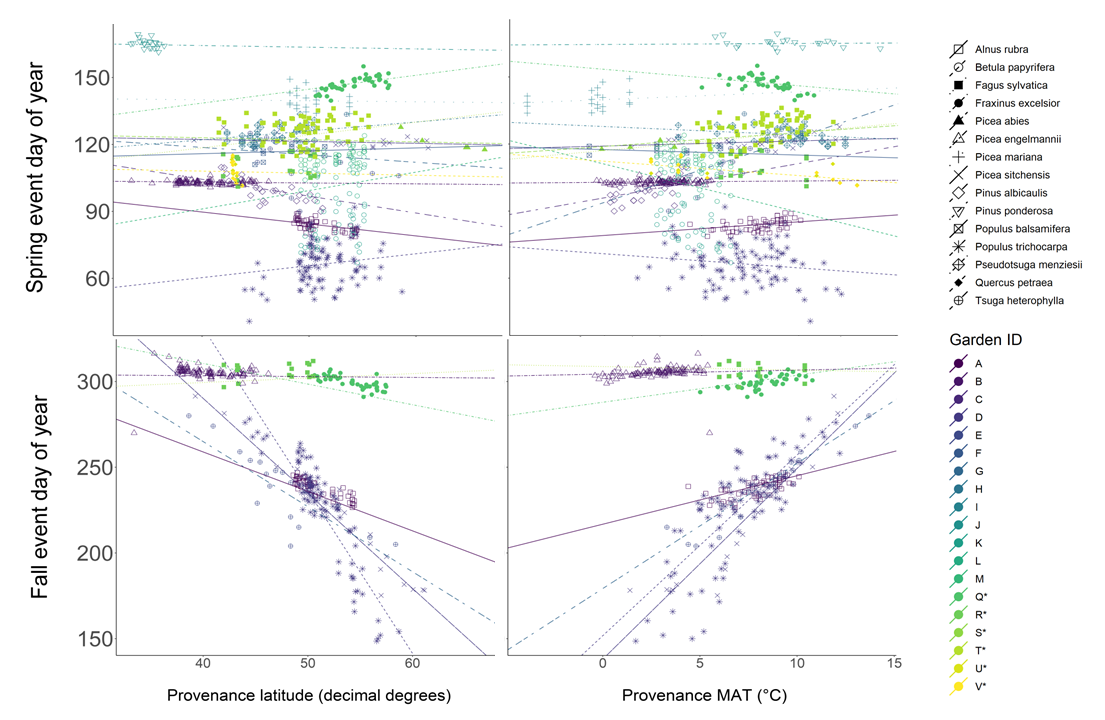
\includegraphics[width=\textwidth]{..//..//localadaptclim/Docs/figure_ms/springfall_latmat.jpg}
    \caption{Event day of year (DOY) in relation to provenance latitude and MAT, coded by symbol for species and color for garden with linear fits from hierarchical Bayesian models. Spring events shown on top and fall events at the bottom. European Gardens and species are bolded and denoted by an asterisk (*). } 
    \label{figure:springfall_latmat}
\end{figure}


In contrast, fall events (budset, leaf senescence, leaf abscission) advanced strongly with provenance latitude (3.16 days/degree [2.87-3.45]) and the decrease in MAT (4.78 days/$^{\circ}$C [4.1 - 5.4]), meaning fall events WEre earlier where provenance MAT was lower (Fig. \ref{figure:springfall_latmat}, Table.\ref{supplement-table:model_fall_lat} \& \ref{supplement-table:model_fall_mat} in Supplements ). This relationship, however, was observed mostly in North America where fall events advanced 4.24 (3.95 - 4.53) days per degree northward, or 6.41 days (5.78 - 7.04) per degree decline in MAT ($^{\circ}$C), whereas in Europe these relationships were weaker: advance of 0.47 (0.21 - 1.17) days per degree northward, or 0.70 days (1.04 - 2.42) per degree decline in MAT $^{\circ}$C(Fig. \ref{figure:continental_spptype_effect}A). \\

\begin{figure}[!h] 
    \centering
 \includegraphics[width=\textwidth]{..//..//localadaptclim/Docs/figure_ms/continental_spptype_effect.jpg}
    \caption{Posterior distributions for the effect of MAT across different continents and species types. Zero -- no effect -- is shown with a dashed line. Solid line and shading in posteriors represent mean and 50 percent interval. (A) Effect of MAT and continent on spring and fall event date (DOY). Fall events advanced strongly with decreasing MAT, particularly notably in North America. Effect of MAT and leaf type on spring and fall event date (DOY) weakly diverged. (B) Effect of MAT and leaf type on spring and fall event date (DOY). As MAT increased, spring events slightly advanced in angiosperms and delayed in gymnosperms. Fall events delayed in warmer locations for both species types.}
    \label{figure:continental_spptype_effect}
\end{figure}

Effects of provenance latitude on both spring and fall events were similar across angiosperms and gymnosperms.
Spring events slightly delayed 0.37 (0.15 - 0.59) days per degree north in angiosperms and 0.23 (0.00 - 0.46) days per degree north in gymnosperms. Fall events advanced 3.18 (2.76 - 3.62) days per degree north in angiosperms and 3.14 (2.81-3.47) days per degree north in gymnosperms.
However, effects of MAT on spring events weakly diverged (Fig.\ref{figure:continental_spptype_effect}B). Spring events advanced 0.82 (0.54 - 1.11) days/$^{\circ}$C as MAT increased in angiosperms and delayed 0.76 (0.37 - 1.14) days/$^{\circ}$C as MAT increased in gymnosperms. Fall events delayed in warmer locations for both species types, but slightly more so for gymnosperms (6.23 days) than angiosperms (3.69 days) (Fig. \ref{figure:continental_spptype_effect}B).\\

%EMWApr20 -- need to refer to some supp figures or tables or such below. Once you have the supp so I can see better what we're referring to here in first sentence we should likely edit this paragraph a little. 
While we believe that coarse metrics such as latitude and MAT would ultimately represent how similar the climates are between the provenances and gardens, we also estimated climate overlap in months that matter for the events to further test how much climate similarity between provenances and gardens predicts local adaptation. For spring events, we considered overlap across March to May. However, results were not qualitatively different than using MAT (See Fig. \ref{supplement-figure:overlap_scatterplot} in Supplements). We observed very weak effects of climate overlap on spring events (0.01 [0.02 - 0.03] days per one per cent increase in climate overlap), nearly identical across angiosperms (0.02 [0.00 - 0.05]) and gymnosperms (0.04 [0.00 - 0.09]). Fall events advanced as climate overlap declined, but slightly more strongly for gymnosperms (advancing 0.72 [0.51 - 0.92] days per one per cent decline in climate overlap) (Fig.\ref{supplement-figure:overlap_posterior} in Supplements).



% old graphs can be found in C:\Users\alina\Documents\git\localadaptclim\Output\plotMay15_two predictors_experiment
% refer to analyses\script_model_continent_spp_type_effect
% https://github.com/lizzieinvancouver/localadaptclim/issues/16



\section{Discussion}
%emw2Mar -- there's a delicate balance of how much rationale you can give for your methods in the methods (and similar for the results). I would move the below to the discussion section. 
While coarse metrics such as latitude and MAT may represent how similar the climates are between the provenances and gardens in times that matter for the events. If climates are very similar, then we would expect similar timings [add more here].

%emw2Mar -- save the below for now; may fit in the discussion or could add if reveiwers complain. For now, I added the events above -- it's quicker and IMHO we don't currently need to justify why we pooled these. 
We pooled the timing of budburst and leaf flush into a single category of ‘spring events’ and the timing of bud set, leaf senescence, growth cessation, and leaf abscission into ‘fall events.’ Such pooling is justified because of the shared pressures from natural selection that govern these events \citep{Gill15}. 

The weak relationship between spring event dates and provenance latitude and MAT that we find in European studies might be explained by the higher extent of climate overlap in those studies. The more similar the climate is between provenances and gardens, the less difference between spring event dates.
\\

The inconsistent and weak clines in spring events that we found suggest high plasticity in spring phenology across continents and species. Fall events, on the other hand, exhibit stronger clines which suggest more local adaptation, especially in North America. Overall, our results predict that warming springs will continue to be tracked more closely phenologically by trees than warming fall temperatures.
\\

In contrast to spring events, we found strong latitudinal clines in fall events across both continents, with local adaptation appearing much stronger in North America than in Europe. Our results show that spring events are highly plastic, and thus may shift with warming, but data on more species and greater information on important factors, such as their geographic location in relation to their origins and elevation, are needed for forecasting. 


% Must cover in discussion:

% Counter vs. co gradient literature
% Maybe also discuss? ice sheet dynamics in Europe/North America, which could impact rates of local adaptation.





\section{Figures}



\bibliography{bibliography_local_adaptation.bib}



\section{Acknowledgement}
We thank S. Aitken,  I. Chuine, R. Guy, C Korner and Y. Vitasse for reviewing our list of papers for possible additional common garden studies. 


\end{document}




% helping with abstract language
% Alberto16
% "On the basis of the patterns of quantitative variation for 19 adaptation-related traits studied in 59 tree species (mostly temperate and boreal species from the Northern hemisphere), we found that genetic differentiation between populations and clinal variation along environmental gradients were very common (respectively, 90% and 78% of cases)."

% formatting code resources
% https://github.com/lizzieinvancouver/ospree/blob/master/docs/ranges/ranges_outline.tex
% https://github.com/lizzieinvancouver/ospree/blob/master/docs/traits/Traitors_Manuscript_supp.Rnw

